% What is built with what in stdlib_Integrate: the dependency graph inverted
% and drawn at the level of types and procedures. The primitives (no
% dependency inside the library) are at the top; an arrow goes from a
% building block to what is built with it, so each primitive's arrows, in its
% own colour, show everything that uses it. status_t (used by everything)
% and stdlib_kinds are left out. Dashed: the descriptor only (read once at
% init), not the coefficients.
\documentclass[tikz,border=6pt]{standalone}
\usetikzlibrary{arrows.meta,positioning,fit,backgrounds}

% Palette: one colour per building block, for its arrows; boxes grey, the entry point blue.
\definecolor{handcol}{RGB}{235,235,235}
\definecolor{topcol}{RGB}{214,230,245}
\definecolor{cstage}{RGB}{31,119,180}
\definecolor{cmethod}{RGB}{44,160,44}
\definecolor{ckern}{RGB}{148,103,189}
\definecolor{cctrl}{RGB}{214,39,40}
\definecolor{cmodel}{RGB}{90,90,90}
\definecolor{ctab}{RGB}{214,120,0}
\definecolor{cif}{RGB}{23,170,190}
\definecolor{cscheme}{RGB}{0,0,0}
\definecolor{cbuf}{RGB}{140,86,75}

% What a block is, in small italics under its name.
\newcommand{\what}[1]{{\footnotesize\rmfamily\itshape\color{black!65}#1}}

\begin{document}
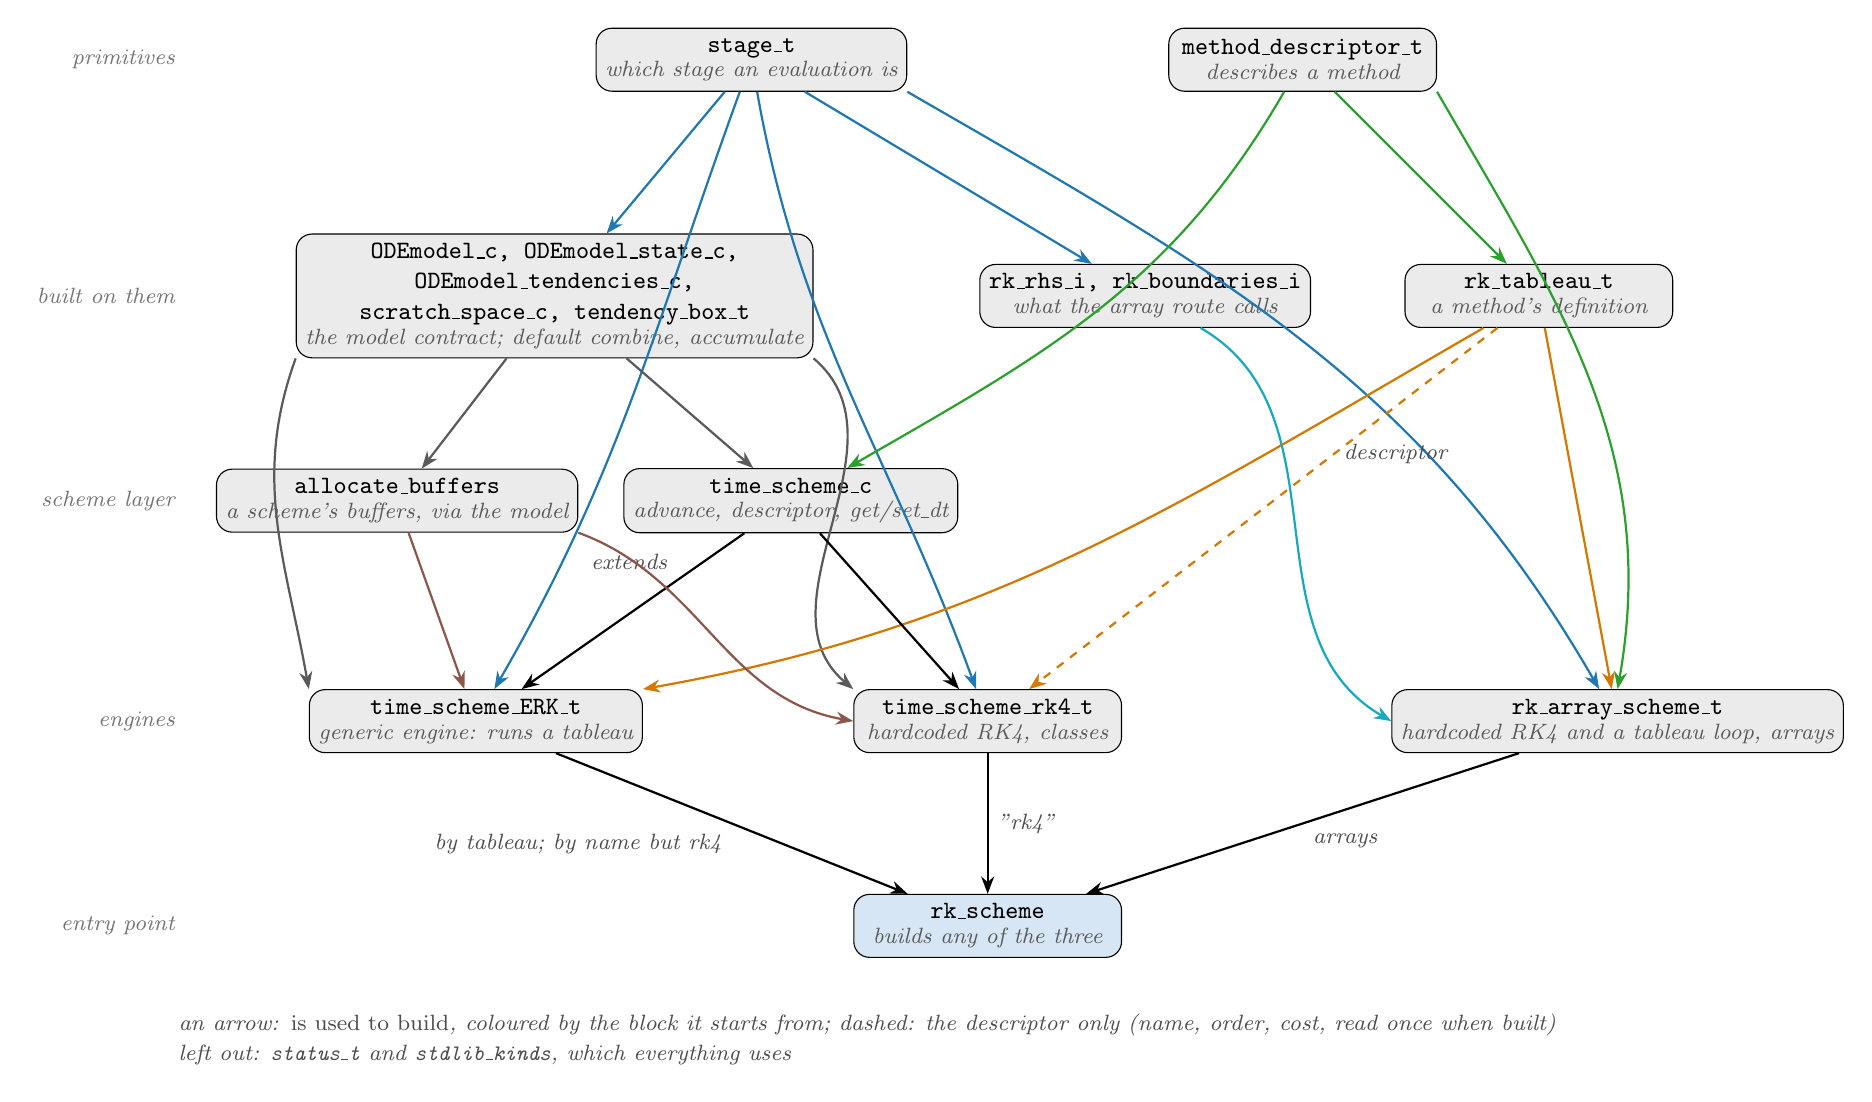
\begin{tikzpicture}[
    font=\small,
    >={Stealth[length=2.2mm]},
    blk/.style={draw, rounded corners=2mm, fill=handcol, minimum height=8mm,
                minimum width=34mm, align=center, font=\small\ttfamily},     % a type or procedure
    entry/.style={blk, fill=topcol},                                        % what a program calls
    built/.style={->, thick},                                               % "is used to build"
    meta/.style={->, thick, dashed},                                        % metadata only
    row/.style={font=\footnotesize\itshape, text=black!55, anchor=east},    % row label
    note/.style={font=\footnotesize\itshape, text=black!70, align=left},     % explanatory note
  ]

  % ---- primitives: nothing inside the library ----
  \node[blk] (stage)  at (5, 12)    {stage\_t\\[-2pt]\what{which stage an evaluation is}};
  \node[blk] (method) at (12, 12)   {method\_descriptor\_t\\[-2pt]\what{describes a method}};

  % ---- built on primitives only ----
  \node[blk, minimum width=44mm] (model) at (2.5, 9)
       {ODEmodel\_c, ODEmodel\_state\_c,\\ODEmodel\_tendencies\_c,\\scratch\_space\_c, tendency\_box\_t\\[-2pt]
        \what{the model contract; default combine, accumulate}};
  \node[blk] (ifs)    at (10, 9)   {rk\_rhs\_i, rk\_boundaries\_i\\[-2pt]\what{what the array route calls}};
  \node[blk] (tab)    at (15, 9)  {rk\_tableau\_t\\[-2pt]\what{a method's definition}};

  % ---- the scheme layer ----
  \node[blk] (buf)    at (0.5, 6.4) {allocate\_buffers\\[-2pt]\what{a scheme's buffers, via the model}};
  \node[blk] (scheme) at (5.5, 6.4) {time\_scheme\_c\\[-2pt]\what{advance, descriptor, get/set\_dt}};

  % ---- the engines ----
  \node[blk] (erk)    at (1.5, 3.6) {time\_scheme\_ERK\_t\\[-2pt]\what{generic engine: runs a tableau}};
  \node[blk] (rk)     at (8, 3.6)   {time\_scheme\_rk4\_t\\[-2pt]\what{hardcoded RK4, classes}};
  \node[blk] (arr)    at (16, 3.6)  {rk\_array\_scheme\_t\\[-2pt]\what{hardcoded RK4 and a tableau loop, arrays}};

  % ---- entry point ----
  \node[entry] (ctor) at (8, 1)     {rk\_scheme\\[-2pt]\what{builds any of the three}};

  % ---- row labels ----
  \foreach \y/\t in {12/primitives, 9/built on them, 6.4/scheme layer, 3.6/engines, 1/entry point} {
    \node[row] at (-2.2, \y) {\t};
  }

  % ---- stage_t ----
  \draw[built, cstage] (stage) -- (model);
  \draw[built, cstage] (stage) -- (ifs);
  \draw[built, cstage] (stage) to[out=-110, in=60] (erk);
  \draw[built, cstage] (stage) to[out=-80, in=110] (rk);
  \draw[built, cstage] (stage.south east) to[out=-30, in=120] (arr);

  % ---- method_descriptor_t ----
  \draw[built, cmethod] (method) -- (tab);
  \draw[built, cmethod] (method) to[out=-120, in=30] (scheme);
  \draw[built, cmethod] (method.south east) to[out=-60, in=80] (arr.north);

  % ---- the model contract ----
  \draw[built, cmodel] (model) -- (buf);
  \draw[built, cmodel] (model) -- (scheme);
  \draw[built, cmodel] (model.south west) to[out=-110, in=100] (erk.north west);
  \draw[built, cmodel] (model.south east) to[out=-40, in=140] (rk.north west);

  % ---- rk_tableau_t: run by the generic engine and the array loop, read for metadata by the RK4 step ----
  \draw[built, ctab] (tab) to[out=-150, in=10] (erk.north east);
  \draw[meta, ctab] (tab) -- node[note, right, pos=0.35] {descriptor} (rk);
  \draw[built, ctab] (tab) -- (arr);

  % ---- the array route's interfaces ----
  \draw[built, cif] (ifs) to[out=-30, in=150] (arr.west);

  % ---- the scheme layer into the engines ----
  \draw[built, cscheme] (scheme) -- node[note, above left, pos=0.3] {extends} (erk);
  \draw[built, cscheme] (scheme) -- (rk);
  \draw[built, cbuf] (buf) -- (erk);
  \draw[built, cbuf] (buf.south east) to[out=-20, in=170] (rk.west);

  % ---- the engines into the entry point ----
  \draw[built] (erk) -- node[note, below left] {by tableau; by name but rk4} (ctor);
  \draw[built] (rk)  -- node[note, right] {"rk4"} (ctor);
  \draw[built] (arr) -- node[note, below right] {arrays} (ctor);

  % ---- legend ----
  \node[note, anchor=north west] at (-2.4, 0)
       {an arrow: \emph{is used to build}, coloured by the block it starts from;
        dashed: the descriptor only (name, order, cost, read once when built)\\[1pt]
        left out: \texttt{status\_t} and \texttt{stdlib\_kinds}, which everything uses};
\end{tikzpicture}
\end{document}
